\chapter{EKSPERIMEN DAN ANALISIS}

\section{LINGKUNGAN PENGUJIAN}

Pengujian sistem dilakukan setelah tahap implementasi selesai dilaksanakan. Pengujian bertujuan untuk memastikan bahwa seluruh fungsionalitas sistem manajemen Praktik Kerja Lapangan (PKL) berbasis web InternSync telah berjalan sesuai dengan perancangan dan kebutuhan pengguna di SMK PGRI Telagasari.

Metode pengujian yang digunakan adalah Black Box Testing, yaitu pengujian yang berfokus pada validasi input dan output sistem dari perspektif pengguna akhir tanpa memperhatikan struktur kode internal. Sistem telah di-deploy dan dapat diakses secara publik. Lingkungan pengujian yang digunakan disajikan pada Tabel 4.1.

{\singlespacing\small\renewcommand{\arraystretch}{1.25}
\begin{longtable}{|>{\raggedright\arraybackslash}p{\dimexpr(\linewidth-3\arrayrulewidth)*2225/7938-2\tabcolsep\relax}|>{\raggedright\arraybackslash}p{\dimexpr(\linewidth-3\arrayrulewidth)*5713/7938-2\tabcolsep\relax}|}
\caption{Lingkungan Pengujian Sistem}\label{tab:4.1}\\
\hline
\rowcolor[HTML]{D9D9D9}\multicolumn{1}{|>{\centering\arraybackslash\bfseries}p{\dimexpr(\linewidth-3\arrayrulewidth)*2225/7938-2\tabcolsep\relax}|}{Komponen} & \multicolumn{1}{|>{\centering\arraybackslash\bfseries}p{\dimexpr(\linewidth-3\arrayrulewidth)*5713/7938-2\tabcolsep\relax}|}{Spesifikasi} \\ \hline
\endfirsthead
\hline
\rowcolor[HTML]{D9D9D9}\multicolumn{1}{|>{\centering\arraybackslash\bfseries}p{\dimexpr(\linewidth-3\arrayrulewidth)*2225/7938-2\tabcolsep\relax}|}{Komponen} & \multicolumn{1}{|>{\centering\arraybackslash\bfseries}p{\dimexpr(\linewidth-3\arrayrulewidth)*5713/7938-2\tabcolsep\relax}|}{Spesifikasi} \\ \hline
\endhead
Browser & Google Chrome (versi terbaru) \\ \hline
Sistem Operasi Server & Ubuntu 24.04 LTS \\ \hline
Backend Framework & Laravel (PHP) \\ \hline
Frontend Framework & React.js \\ \hline
Database & MySQL \\ \hline
Metode Pengujian & Black Box Testing \\ \hline
Hosting & CloudPanel \\ \hline
CDN / Proxy & Cloudflare \\ \hline
Domain Sistem & internsync.smkpgritelagasari.sch.id \\ \hline
Jaringan Pengujian & Jaringan internet (akses publik) \\ \hline
\end{longtable}}

\section{PARAMETER PENGUJIAN}

Pengujian sistem InternSync dilakukan terhadap sembilan parameter utama yang mencakup seluruh skenario penggunaan oleh masing-masing aktor sistem, pengujian keamanan akses, penanganan kesalahan, responsivitas antarmuka, serta evaluasi kepuasan pengguna melalui kuesioner. Parameter-parameter tersebut adalah:

\begin{enumerate}[label=\arabic*.]
\item Pengujian fungsionalitas sebagai Siswa
\item Pengujian fungsionalitas sebagai Guru Pembimbing
\item Pengujian fungsionalitas sebagai Koordinator PKL
\item Pengujian fungsionalitas sebagai Hubin (Hubungan Industri)
\item Pengujian fungsionalitas sebagai Admin Sistem
\item Pengujian keamanan akses (Role-Based Access Control)
\item Pengujian penanganan kesalahan (Error Handling)
\item Pengujian responsivitas antarmuka
\item Pengujian melalui penyebaran kuesioner kepuasan pengguna
\end{enumerate}

\section{HASIL IMPLEMENTASI ANTARMUKA SISTEM}

Subbab ini mendokumentasikan antarmuka InternSync yang telah diimplementasikan melalui tangkapan layar aplikasi. Gambar disusun menurut alur penggunaan dan dikelompokkan berdasarkan peran pengguna. Dua gambar autentikasi ditampilkan terlebih dahulu karena digunakan bersama oleh seluruh peran, kemudian diikuti antarmuka Siswa, Guru Pembimbing, Koordinator PKL, Hubin, dan Admin Sistem.

\newcommand{\antarmukagambar}[4]{%
\begin{figure}[H]
\centering
\includegraphics[width=0.98\linewidth,height=0.58\textheight,keepaspectratio]{#1}
\caption{#2}\label{#3}
\end{figure}
#4\par\medskip}

\antarmukagambar{gambar/auth/01_Auth_SignIn.png}{Halaman Masuk InternSync}{fig:ui-auth-signin}{Halaman masuk menjadi gerbang autentikasi bagi pengguna sebelum mengakses fitur sesuai perannya.}

\antarmukagambar{gambar/auth/02_Auth_ForgotPassword.png}{Halaman Pemulihan Kata Sandi}{fig:ui-auth-forgot-password}{Halaman ini menyediakan alur pemulihan kata sandi melalui alamat email pengguna.}

\subsection{Antarmuka Pengguna Siswa}

Antarmuka Siswa mendukung kebutuhan siswa selama mengikuti PKL, mulai dari melihat informasi, memeriksa penempatan, mencatat kegiatan, mengajukan izin, hingga melihat hasil evaluasi.

\antarmukagambar{gambar/siswa/01_Siswa_Dashboard.png}{Dasbor Siswa}{fig:ui-siswa-dashboard}{Dasbor merangkum aktivitas logbook dan progres pelaksanaan PKL siswa.}

\antarmukagambar{gambar/siswa/02_Siswa_Vacancies.png}{Katalog Lowongan PKL}{fig:ui-siswa-vacancies}{Halaman ini menampilkan katalog lowongan PKL yang dapat ditinjau siswa.}

\antarmukagambar{gambar/siswa/03_Siswa_Placement.png}{Informasi Penempatan PKL Siswa}{fig:ui-siswa-placement}{Halaman penempatan memperlihatkan informasi industri dan periode pelaksanaan PKL siswa.}

\antarmukagambar{gambar/siswa/04_Siswa_Logbook.png}{Daftar Logbook Harian Siswa}{fig:ui-siswa-logbook}{Siswa menggunakan halaman ini untuk melihat catatan kegiatan harian dan mengakses pencatatan logbook.}

\antarmukagambar{gambar/siswa/05_Siswa_Permissions.png}{Riwayat Pengajuan Izin dan Sakit Siswa}{fig:ui-siswa-permissions}{Halaman ini menampilkan daftar pengajuan izin atau sakit beserta statusnya.}

\antarmukagambar{gambar/siswa/06_Siswa_Evaluation.png}{Hasil Evaluasi dan Nilai Akhir PKL Siswa}{fig:ui-siswa-evaluation}{Halaman evaluasi menyajikan nilai akhir dan rincian aspek penilaian PKL siswa.}

\antarmukagambar{gambar/siswa/07_Siswa_Profile.png}{Profil Pengguna Siswa}{fig:ui-siswa-profile}{Halaman profil menampilkan informasi akun dan data pribadi siswa.}

\subsection{Antarmuka Guru Pembimbing}

Antarmuka Guru Pembimbing berfokus pada pemantauan siswa bimbingan, pemeriksaan logbook dan izin, evaluasi, serta informasi kunjungan industri.

\antarmukagambar{gambar/pembimbing/01_Pembimbing_Dashboard.png}{Dasbor Guru Pembimbing}{fig:ui-pembimbing-dashboard}{Dasbor menyajikan ringkasan siswa bimbingan, aktivitas, dan pemantauan PKL.}

\antarmukagambar{gambar/pembimbing/02_Pembimbing_Supervisions.png}{Daftar Siswa Bimbingan}{fig:ui-pembimbing-supervisions}{Halaman ini menampilkan siswa yang berada dalam bimbingan beserta informasi penempatannya.}

\antarmukagambar{gambar/pembimbing/03_Pembimbing_LogbookMonitoring.png}{Pemantauan Logbook Siswa}{fig:ui-pembimbing-logbook}{Guru Pembimbing menggunakan halaman ini untuk memeriksa catatan kegiatan harian siswa bimbingan.}

\antarmukagambar{gambar/pembimbing/04_Pembimbing_Permissions.png}{Verifikasi Pengajuan Izin dan Sakit}{fig:ui-pembimbing-permissions}{Halaman verifikasi menampilkan pengajuan izin atau sakit siswa untuk ditinjau berdasarkan statusnya.}

\antarmukagambar{gambar/pembimbing/05_Pembimbing_Evaluations.png}{Pemantauan Evaluasi Siswa}{fig:ui-pembimbing-evaluations}{Halaman ini menampilkan daftar siswa dan informasi penilaian yang perlu dipantau Guru Pembimbing.}

\antarmukagambar{gambar/pembimbing/06_Pembimbing_IndustryVisits.png}{Jadwal Kunjungan Industri}{fig:ui-pembimbing-industry-visits}{Guru Pembimbing dapat melihat jadwal kunjungan industri yang terkait dengan siswa bimbingan.}

\antarmukagambar{gambar/pembimbing/07_Pembimbing_Profile.png}{Profil Pengguna Guru Pembimbing}{fig:ui-pembimbing-profile}{Halaman profil menampilkan informasi akun dan data Guru Pembimbing.}

\subsection{Antarmuka Koordinator PKL}

Antarmuka Koordinator PKL mendukung pengelolaan lowongan dan proses penempatan, serta pemantauan kunjungan dan rekapitulasi pelaksanaan PKL.

\antarmukagambar{gambar/koordinator/01_Koordinator_Dashboard.png}{Dasbor Koordinator PKL}{fig:ui-koordinator-dashboard}{Dasbor merangkum data siswa, lowongan, industri, dan status pelaksanaan PKL.}

\antarmukagambar{gambar/koordinator/02_Koordinator_Vacancies.png}{Pengelolaan Lowongan PKL}{fig:ui-koordinator-vacancies}{Halaman ini digunakan untuk melihat dan mengelola data lowongan PKL.}

\antarmukagambar{gambar/koordinator/03_Koordinator_Applications.png}{Daftar Pengajuan Penempatan PKL}{fig:ui-koordinator-applications}{Halaman Pengajuan PKL menampilkan daftar perusahaan tujuan, pembimbing, jumlah siswa, periode pengajuan, dan status surat penempatan.}

\antarmukagambar{gambar/koordinator/04_Koordinator_Placements.png}{Daftar Pengiriman PKL}{fig:ui-koordinator-placements}{Halaman Pengiriman PKL menampilkan daftar batch siswa, pembimbing, tanggal keberangkatan, dan status pengiriman ke industri.}

\antarmukagambar{gambar/koordinator/05_Koordinator_PlacementsHistory.png}{Riwayat Penempatan PKL}{fig:ui-koordinator-placement-history}{Riwayat ini memperlihatkan data penempatan PKL beserta status dan tindak lanjutnya.}

\antarmukagambar{gambar/koordinator/06_Koordinator_Monitoring.png}{Pengelolaan Kunjungan Industri}{fig:ui-koordinator-monitoring}{Koordinator dapat memantau data kunjungan industri dan status persetujuannya.}

\antarmukagambar{gambar/koordinator/07_Koordinator_SummaryReports.png}{Rekapitulasi dan Laporan PKL}{fig:ui-koordinator-reports}{Halaman rekapitulasi menyajikan data siswa dan status akhir pelaksanaan PKL.}

\antarmukagambar{gambar/koordinator/08_Koordinator_Profile.png}{Profil Pengguna Koordinator PKL}{fig:ui-koordinator-profile}{Halaman profil menampilkan informasi akun dan data Koordinator PKL.}

\subsection{Antarmuka Hubin}

Antarmuka Hubin mendukung pengelolaan mitra industri serta peninjauan dan persetujuan pengajuan PKL, penempatan siswa, dan kunjungan industri.

\antarmukagambar{gambar/hubin/01_Hubin_Dashboard.png}{Dasbor Hubin}{fig:ui-hubin-dashboard}{Dasbor menampilkan ringkasan mitra industri dan status pengajuan yang memerlukan perhatian.}

\antarmukagambar{gambar/hubin/02_Hubin_Industries.png}{Pengelolaan Mitra Industri}{fig:ui-hubin-industries}{Halaman ini menampilkan daftar mitra industri dan informasi terkait.}

\antarmukagambar{gambar/hubin/03_Hubin_Persetujuan_Pengajuan.png}{Persetujuan Pengajuan PKL}{fig:ui-hubin-applications}{Hubin meninjau pengajuan PKL dari Koordinator sebelum memberikan keputusan.}

\antarmukagambar{gambar/hubin/04_Hubin_Persetujuan_Penempatan.png}{Persetujuan Pengiriman dan Penempatan Siswa}{fig:ui-hubin-placements}{Halaman ini digunakan Hubin untuk meninjau proses pengiriman dan penempatan siswa PKL.}

\antarmukagambar{gambar/hubin/05_Hubin_Persetujuan_Kunjungan.png}{Persetujuan Kunjungan Industri}{fig:ui-hubin-visits}{Hubin dapat meninjau permohonan kunjungan industri pada halaman ini.}

\antarmukagambar{gambar/hubin/06_Hubin_MasterReports.png}{Laporan Rekapitulasi PKL Hubin}{fig:ui-hubin-reports}{Halaman laporan merangkum data pelaksanaan PKL dan distribusi penempatan siswa.}

\antarmukagambar{gambar/hubin/07_Hubin_Profile.png}{Profil Pengguna Hubin}{fig:ui-hubin-profile}{Halaman profil menampilkan informasi akun dan data pengguna Hubin.}

\subsection{Antarmuka Admin Sistem}

Antarmuka Admin Sistem menyediakan fungsi administrasi akun, data master, pengaturan aplikasi, dan peninjauan aktivitas sistem.

\antarmukagambar{gambar/admin/01_Admin_Dashboard.png}{Dasbor Admin Sistem}{fig:ui-admin-dashboard}{Dasbor memberikan ringkasan data dan aktivitas administrasi sistem.}

\antarmukagambar{gambar/admin/02_Admin_UserManagement.png}{Manajemen Pengguna}{fig:ui-admin-users}{Halaman ini digunakan untuk melihat dan mengelola data akun pengguna.}

\antarmukagambar{gambar/admin/03_Admin_DataMaster.png}{Pengelolaan Data Master Sekolah}{fig:ui-admin-master-data}{Admin dapat mengelola data master sekolah yang digunakan dalam proses PKL.}

\antarmukagambar{gambar/admin/04_Admin_SystemSetting.png}{Pengaturan Global Sistem}{fig:ui-admin-settings}{Halaman pengaturan memuat konfigurasi identitas dan informasi sistem.}

\antarmukagambar{gambar/admin/05_Admin_ActivityLogs.png}{Log Aktivitas Admin}{fig:ui-admin-activity-logs}{Log aktivitas menyajikan catatan kegiatan administratif yang tercatat di sistem.}

\antarmukagambar{gambar/admin/06_Admin_Profile.png}{Profil Pengguna Admin}{fig:ui-admin-profile}{Halaman profil menampilkan informasi akun dan data Admin Sistem.}

\section{HASIL PENGUJIAN FUNGSIONALITAS PER PERAN PENGGUNA}

\subsection{PENGUJIAN SEBAGAI SISWA}

Pengujian pada peran Siswa bertujuan untuk memverifikasi seluruh fitur yang dapat diakses selama pelaksanaan PKL, mulai dari melihat dan memilih lowongan, melihat data penempatan, pengelolaan logbook harian, hingga melihat nilai akhir. Hasil pengujian disajikan pada Tabel~\ref{tab:4.2}.

{\singlespacing\small\renewcommand{\arraystretch}{1.25}
\begin{longtable}{|>{\raggedright\arraybackslash}p{\dimexpr(\linewidth-5\arrayrulewidth)*511/7938-2\tabcolsep\relax}|>{\raggedright\arraybackslash}p{\dimexpr(\linewidth-5\arrayrulewidth)*3034/7938-2\tabcolsep\relax}|>{\raggedright\arraybackslash}p{\dimexpr(\linewidth-5\arrayrulewidth)*1359/7938-2\tabcolsep\relax}|>{\raggedright\arraybackslash}p{\dimexpr(\linewidth-5\arrayrulewidth)*3034/7938-2\tabcolsep\relax}|}
\caption{Hasil Pengujian Fungsionalitas Peran Siswa}\label{tab:4.2}\\
\hline
\rowcolor[HTML]{D9D9D9}\multicolumn{1}{|>{\centering\arraybackslash\bfseries}p{\dimexpr(\linewidth-5\arrayrulewidth)*511/7938-2\tabcolsep\relax}|}{No} & \multicolumn{1}{|>{\centering\arraybackslash\bfseries}p{\dimexpr(\linewidth-5\arrayrulewidth)*3034/7938-2\tabcolsep\relax}|}{Fitur yang Diuji} & \multicolumn{1}{|>{\centering\arraybackslash\bfseries}p{\dimexpr(\linewidth-5\arrayrulewidth)*1359/7938-2\tabcolsep\relax}|}{Hasil} & \multicolumn{1}{|>{\centering\arraybackslash\bfseries}p{\dimexpr(\linewidth-5\arrayrulewidth)*3034/7938-2\tabcolsep\relax}|}{Keterangan} \\ \hline
\endfirsthead
\hline
\rowcolor[HTML]{D9D9D9}\multicolumn{1}{|>{\centering\arraybackslash\bfseries}p{\dimexpr(\linewidth-5\arrayrulewidth)*511/7938-2\tabcolsep\relax}|}{No} & \multicolumn{1}{|>{\centering\arraybackslash\bfseries}p{\dimexpr(\linewidth-5\arrayrulewidth)*3034/7938-2\tabcolsep\relax}|}{Fitur yang Diuji} & \multicolumn{1}{|>{\centering\arraybackslash\bfseries}p{\dimexpr(\linewidth-5\arrayrulewidth)*1359/7938-2\tabcolsep\relax}|}{Hasil} & \multicolumn{1}{|>{\centering\arraybackslash\bfseries}p{\dimexpr(\linewidth-5\arrayrulewidth)*3034/7938-2\tabcolsep\relax}|}{Keterangan} \\ \hline
\endhead
1 & Login ke sistem menggunakan email dan kata sandi & Berhasil & Sistem mengarahkan ke dasbor siswa sesuai role \\ \hline
2 & Melihat data penempatan PKL (industri, durasi, pembimbing) & Berhasil & Informasi penempatan tampil lengkap dan akurat \\ \hline
3 & Melihat katalog lowongan PKL (industri, posisi, deskripsi, kuota, jenis lowongan) & Berhasil & Lowongan yang dibuat koordinator tampil lengkap sesuai ketentuan jenis lowongan \\ \hline
4 & Memilih lowongan PKL & Berhasil & Pilihan tersimpan dengan status menunggu seleksi koordinator \\ \hline
5 & Mengunduh surat pengantar dan penempatan PKL & Berhasil & File surat dinas berhasil diunduh dalam format PDF \\ \hline
6 & Mengisi dan mengelola logbook harian beserta lampiran bukti & Berhasil & Data aktivitas tersimpan mandiri dan tercatat secara kronologis \\ \hline
7 & Mengajukan izin dan sakit dengan melampirkan berkas bukti sah & Berhasil & Data izin tersimpan dan tautan konfirmasi terkirim ke industri \\ \hline
8 & Melihat progres PKL melalui gauge chart pada dasbor & Berhasil & Persentase progres terhitung otomatis berdasarkan durasi hari \\ \hline
9 & Melihat hasil evaluasi dan nilai akhir berbasis rubrik baku & Berhasil & Nilai rubrik ditampilkan dan lembar penilaian PDF dapat diunduh \\ \hline
10 & Logout dari sistem & Berhasil & Sesi berakhir dan pengguna diarahkan ke halaman login \\ \hline
\end{longtable}}

\subsection{PENGUJIAN SEBAGAI GURU PEMBIMBING}

Pengujian pada peran Guru Pembimbing difokuskan pada kemampuan sistem dalam memfasilitasi aktivitas pengawasan, pemantauan logbook, verifikasi izin, serta rekapitulasi penilaian kinerja siswa yang berada di bawah supervisinya. Hasil pengujian disajikan pada Tabel~\ref{tab:4.3}.

{\singlespacing\small\renewcommand{\arraystretch}{1.25}
\begin{longtable}{|>{\raggedright\arraybackslash}p{\dimexpr(\linewidth-5\arrayrulewidth)*501/7938-2\tabcolsep\relax}|>{\raggedright\arraybackslash}p{\dimexpr(\linewidth-5\arrayrulewidth)*3113/7938-2\tabcolsep\relax}|>{\raggedright\arraybackslash}p{\dimexpr(\linewidth-5\arrayrulewidth)*1318/7938-2\tabcolsep\relax}|>{\raggedright\arraybackslash}p{\dimexpr(\linewidth-5\arrayrulewidth)*3006/7938-2\tabcolsep\relax}|}
\caption{Hasil Pengujian Fungsionalitas Peran Guru Pembimbing}\label{tab:4.3}\\
\hline
\rowcolor[HTML]{D9D9D9}\multicolumn{1}{|>{\centering\arraybackslash\bfseries}p{\dimexpr(\linewidth-5\arrayrulewidth)*501/7938-2\tabcolsep\relax}|}{No} & \multicolumn{1}{|>{\centering\arraybackslash\bfseries}p{\dimexpr(\linewidth-5\arrayrulewidth)*3113/7938-2\tabcolsep\relax}|}{Fitur yang Diuji} & \multicolumn{1}{|>{\centering\arraybackslash\bfseries}p{\dimexpr(\linewidth-5\arrayrulewidth)*1318/7938-2\tabcolsep\relax}|}{Hasil} & \multicolumn{1}{|>{\centering\arraybackslash\bfseries}p{\dimexpr(\linewidth-5\arrayrulewidth)*3006/7938-2\tabcolsep\relax}|}{Keterangan} \\ \hline
\endfirsthead
\hline
\rowcolor[HTML]{D9D9D9}\multicolumn{1}{|>{\centering\arraybackslash\bfseries}p{\dimexpr(\linewidth-5\arrayrulewidth)*501/7938-2\tabcolsep\relax}|}{No} & \multicolumn{1}{|>{\centering\arraybackslash\bfseries}p{\dimexpr(\linewidth-5\arrayrulewidth)*3113/7938-2\tabcolsep\relax}|}{Fitur yang Diuji} & \multicolumn{1}{|>{\centering\arraybackslash\bfseries}p{\dimexpr(\linewidth-5\arrayrulewidth)*1318/7938-2\tabcolsep\relax}|}{Hasil} & \multicolumn{1}{|>{\centering\arraybackslash\bfseries}p{\dimexpr(\linewidth-5\arrayrulewidth)*3006/7938-2\tabcolsep\relax}|}{Keterangan} \\ \hline
\endhead
1 & Login dan akses dasbor pembimbing & Berhasil & Dasbor menampilkan ringkasan siswa bimbingan \\ \hline
2 & Melihat daftar siswa bimbingan beserta lokasi industri & Berhasil & Data siswa dikelompokkan per industri disertai progress bar \\ \hline
3 & Memantau logbook harian siswa (monitoring logbook) & Berhasil & Seluruh logbook tampil dengan filter rentang tanggal dan nama siswa \\ \hline
4 & Melihat detail dan file lampiran logbook siswa & Berhasil & File bukti kegiatan dapat dibuka melalui opsi Lihat File \\ \hline
5 & Mengekspor data logbook bimbingan ke format PDF ber-QR Code & Berhasil & File PDF berhasil diunduh memuat rekapitulasi logbook lengkap \\ \hline
6 & Memverifikasi perizinan siswa (verifikasi langsung / fallback) & Berhasil & Status izin diperbarui dan tanggal izin otomatis sinkron ke logbook \\ \hline
7 & Melihat jadwal kunjungan industri dan mengunduh surat tugas (SPPD) & Berhasil & Informasi jadwal dan dokumen SPPD tampil akurat \\ \hline
8 & Merekapitulasi penilaian kinerja siswa berbasis rubrik baku & Berhasil & Nilai rubrik terakumulasi secara otomatis menghasilkan nilai akhir \\ \hline
9 & Melihat rekapitulasi performa keseluruhan siswa bimbingan & Berhasil & Data rekapitulasi siswa bimbingan tampil secara komprehensif \\ \hline
\end{longtable}}

\subsection{PENGUJIAN SEBAGAI KOORDINATOR PKL}

Pengujian pada peran Koordinator PKL mencakup seluruh alur manajerial pengelolaan PKL, mulai dari pengelolaan lowongan dan seleksi siswa, pembuatan pengajuan penempatan, penentuan durasi, hingga pembuatan rekapitulasi laporan akhir. Hasil pengujian disajikan pada Tabel~\ref{tab:4.4}.

{\singlespacing\small\renewcommand{\arraystretch}{1.25}
\begin{longtable}{|>{\raggedright\arraybackslash}p{\dimexpr(\linewidth-5\arrayrulewidth)*506/7937-2\tabcolsep\relax}|>{\raggedright\arraybackslash}p{\dimexpr(\linewidth-5\arrayrulewidth)*3044/7937-2\tabcolsep\relax}|>{\raggedright\arraybackslash}p{\dimexpr(\linewidth-5\arrayrulewidth)*1343/7937-2\tabcolsep\relax}|>{\raggedright\arraybackslash}p{\dimexpr(\linewidth-5\arrayrulewidth)*3044/7937-2\tabcolsep\relax}|}
\caption{Hasil Pengujian Fungsionalitas Peran Koordinator PKL}\label{tab:4.4}\\
\hline
\rowcolor[HTML]{D9D9D9}\multicolumn{1}{|>{\centering\arraybackslash\bfseries}p{\dimexpr(\linewidth-5\arrayrulewidth)*506/7937-2\tabcolsep\relax}|}{No} & \multicolumn{1}{|>{\centering\arraybackslash\bfseries}p{\dimexpr(\linewidth-5\arrayrulewidth)*3044/7937-2\tabcolsep\relax}|}{Fitur yang Diuji} & \multicolumn{1}{|>{\centering\arraybackslash\bfseries}p{\dimexpr(\linewidth-5\arrayrulewidth)*1343/7937-2\tabcolsep\relax}|}{Hasil} & \multicolumn{1}{|>{\centering\arraybackslash\bfseries}p{\dimexpr(\linewidth-5\arrayrulewidth)*3044/7937-2\tabcolsep\relax}|}{Keterangan} \\ \hline
\endfirsthead
\hline
\rowcolor[HTML]{D9D9D9}\multicolumn{1}{|>{\centering\arraybackslash\bfseries}p{\dimexpr(\linewidth-5\arrayrulewidth)*506/7937-2\tabcolsep\relax}|}{No} & \multicolumn{1}{|>{\centering\arraybackslash\bfseries}p{\dimexpr(\linewidth-5\arrayrulewidth)*3044/7937-2\tabcolsep\relax}|}{Fitur yang Diuji} & \multicolumn{1}{|>{\centering\arraybackslash\bfseries}p{\dimexpr(\linewidth-5\arrayrulewidth)*1343/7937-2\tabcolsep\relax}|}{Hasil} & \multicolumn{1}{|>{\centering\arraybackslash\bfseries}p{\dimexpr(\linewidth-5\arrayrulewidth)*3044/7937-2\tabcolsep\relax}|}{Keterangan} \\ \hline
\endhead
1 & Login dan akses dasbor koordinator & Berhasil & Sistem menampilkan dasbor dengan ringkasan metrik PKL \\ \hline
2 & Mengelola lowongan PKL (kuota, jenis umum/khusus, posisi, deskripsi) & Berhasil & Lowongan tersimpan dan tampil pada katalog siswa \\ \hline
3 & Menyeleksi siswa yang memilih lowongan & Berhasil & Hasil seleksi tersimpan dan menjadi dasar pengajuan PKL \\ \hline
4 & Membuat pengajuan penempatan PKL baru (industri, pembimbing, siswa) & Berhasil & Data pengajuan tersimpan dengan status Draft \\ \hline
5 & Menyimpan pengajuan sementara (Simpan Sementara) & Berhasil & Data tersimpan tanpa langsung diteruskan ke Hubin \\ \hline
6 & Mengirim pengajuan PKL secara resmi ke Hubin & Berhasil & Status pengajuan berubah menjadi Menunggu Persetujuan \\ \hline
7 & Mengisi form proses pengiriman PKL (tanggal dan durasi 3/6 bulan) & Berhasil & Data pengiriman tersimpan dan surat pengantar dapat diakses \\ \hline
8 & Mengirim data pengiriman PKL ke Hubin untuk clearance final & Berhasil & Status pengiriman berubah menjadi Menunggu Persetujuan Hubin \\ \hline
9 & Memantau status seluruh pengajuan dan pengiriman PKL & Berhasil & Daftar pengajuan dan status tracking tampil akurat \\ \hline
10 & Mengakses rekapitulasi dan laporan status akhir PKL & Berhasil & Data kumulatif performa siswa tampil lengkap \\ \hline
11 & Mengekspor laporan rekap ke format Excel & Berhasil & File Excel berhasil diunduh memuat data rekapitulasi yang valid \\ \hline
12 & Memfilter rekap berdasarkan jurusan dan status PKL & Berhasil & Data terfilter sesuai parameter jurusan dan status yang dipilih \\ \hline
\end{longtable}}

\subsection{PENGUJIAN SEBAGAI HUBIN}

Pengujian pada peran Hubin difokuskan pada kemampuan sistem dalam mendukung fungsi pengambilan keputusan tingkat sekolah, mencakup persetujuan pengajuan dan pengiriman PKL serta pengelolaan data mitra industri. Hasil pengujian disajikan pada Tabel~\ref{tab:4.5}.

{\singlespacing\small\renewcommand{\arraystretch}{1.25}
\begin{longtable}{|>{\raggedright\arraybackslash}p{\dimexpr(\linewidth-5\arrayrulewidth)*506/7937-2\tabcolsep\relax}|>{\raggedright\arraybackslash}p{\dimexpr(\linewidth-5\arrayrulewidth)*3044/7937-2\tabcolsep\relax}|>{\raggedright\arraybackslash}p{\dimexpr(\linewidth-5\arrayrulewidth)*1343/7937-2\tabcolsep\relax}|>{\raggedright\arraybackslash}p{\dimexpr(\linewidth-5\arrayrulewidth)*3044/7937-2\tabcolsep\relax}|}
\caption{Hasil Pengujian Fungsionalitas Peran Hubin}\label{tab:4.5}\\
\hline
\rowcolor[HTML]{D9D9D9}\multicolumn{1}{|>{\centering\arraybackslash\bfseries}p{\dimexpr(\linewidth-5\arrayrulewidth)*506/7937-2\tabcolsep\relax}|}{No} & \multicolumn{1}{|>{\centering\arraybackslash\bfseries}p{\dimexpr(\linewidth-5\arrayrulewidth)*3044/7937-2\tabcolsep\relax}|}{Fitur yang Diuji} & \multicolumn{1}{|>{\centering\arraybackslash\bfseries}p{\dimexpr(\linewidth-5\arrayrulewidth)*1343/7937-2\tabcolsep\relax}|}{Hasil} & \multicolumn{1}{|>{\centering\arraybackslash\bfseries}p{\dimexpr(\linewidth-5\arrayrulewidth)*3044/7937-2\tabcolsep\relax}|}{Keterangan} \\ \hline
\endfirsthead
\hline
\rowcolor[HTML]{D9D9D9}\multicolumn{1}{|>{\centering\arraybackslash\bfseries}p{\dimexpr(\linewidth-5\arrayrulewidth)*506/7937-2\tabcolsep\relax}|}{No} & \multicolumn{1}{|>{\centering\arraybackslash\bfseries}p{\dimexpr(\linewidth-5\arrayrulewidth)*3044/7937-2\tabcolsep\relax}|}{Fitur yang Diuji} & \multicolumn{1}{|>{\centering\arraybackslash\bfseries}p{\dimexpr(\linewidth-5\arrayrulewidth)*1343/7937-2\tabcolsep\relax}|}{Hasil} & \multicolumn{1}{|>{\centering\arraybackslash\bfseries}p{\dimexpr(\linewidth-5\arrayrulewidth)*3044/7937-2\tabcolsep\relax}|}{Keterangan} \\ \hline
\endhead
1 & Login dan akses dasbor Hubin & Berhasil & Dasbor menampilkan menu persetujuan dan manajemen industri \\ \hline
2 & Melihat detail dokumen pengajuan PKL dari koordinator & Berhasil & Informasi lengkap pengajuan tampil dengan benar \\ \hline
3 & Menyetujui pengajuan PKL dan menerbitkan surat pengantar & Berhasil & Status berubah Disetujui dan surat otomatis diterbitkan \\ \hline
4 & Menolak pengajuan PKL beserta alasan penolakan & Berhasil & Status berubah Ditolak dan koordinator dapat melihat alasan \\ \hline
5 & Melihat detail dokumen pengiriman PKL dari koordinator & Berhasil & Detail pengiriman tampil dengan benar \\ \hline
6 & Menyetujui pengiriman PKL (memicu pembuatan ruang kerja siswa) & Berhasil & Status siswa aktif dan fitur logbook dapat diakses siswa \\ \hline
7 & Menolak pengiriman PKL & Berhasil & Status pengiriman berubah dan koordinator mendapat notifikasi \\ \hline
8 & Mengelola data mitra industri (tambah mitra baru) & Berhasil & Data industri tersimpan dan tersedia bagi koordinator untuk membuat lowongan \\ \hline
9 & Mengedit data mitra industri yang sudah ada & Berhasil & Perubahan data industri tersimpan dengan benar \\ \hline
10 & Melihat seluruh rekapitulasi data PKL & Berhasil & Data rekap dari seluruh siswa tampil secara komprehensif \\ \hline
\end{longtable}}

\subsection{PENGUJIAN SEBAGAI ADMIN SISTEM}

Pengujian pada peran Admin Sistem mencakup fungsionalitas pengelolaan konfigurasi aplikasi dan manajemen data master yang menjadi fondasi operasional sistem secara keseluruhan. Hasil pengujian disajikan pada Tabel~\ref{tab:4.6}.

{\singlespacing\small\renewcommand{\arraystretch}{1.25}
\begin{longtable}{|>{\raggedright\arraybackslash}p{\dimexpr(\linewidth-5\arrayrulewidth)*502/7938-2\tabcolsep\relax}|>{\raggedright\arraybackslash}p{\dimexpr(\linewidth-5\arrayrulewidth)*3055/7938-2\tabcolsep\relax}|>{\raggedright\arraybackslash}p{\dimexpr(\linewidth-5\arrayrulewidth)*1326/7938-2\tabcolsep\relax}|>{\raggedright\arraybackslash}p{\dimexpr(\linewidth-5\arrayrulewidth)*3055/7938-2\tabcolsep\relax}|}
\caption{Hasil Pengujian Fungsionalitas Peran Admin Sistem}\label{tab:4.6}\\
\hline
\rowcolor[HTML]{D9D9D9}\multicolumn{1}{|>{\centering\arraybackslash\bfseries}p{\dimexpr(\linewidth-5\arrayrulewidth)*502/7938-2\tabcolsep\relax}|}{No} & \multicolumn{1}{|>{\centering\arraybackslash\bfseries}p{\dimexpr(\linewidth-5\arrayrulewidth)*3055/7938-2\tabcolsep\relax}|}{Fitur yang Diuji} & \multicolumn{1}{|>{\centering\arraybackslash\bfseries}p{\dimexpr(\linewidth-5\arrayrulewidth)*1326/7938-2\tabcolsep\relax}|}{Hasil} & \multicolumn{1}{|>{\centering\arraybackslash\bfseries}p{\dimexpr(\linewidth-5\arrayrulewidth)*3055/7938-2\tabcolsep\relax}|}{Keterangan} \\ \hline
\endfirsthead
\hline
\rowcolor[HTML]{D9D9D9}\multicolumn{1}{|>{\centering\arraybackslash\bfseries}p{\dimexpr(\linewidth-5\arrayrulewidth)*502/7938-2\tabcolsep\relax}|}{No} & \multicolumn{1}{|>{\centering\arraybackslash\bfseries}p{\dimexpr(\linewidth-5\arrayrulewidth)*3055/7938-2\tabcolsep\relax}|}{Fitur yang Diuji} & \multicolumn{1}{|>{\centering\arraybackslash\bfseries}p{\dimexpr(\linewidth-5\arrayrulewidth)*1326/7938-2\tabcolsep\relax}|}{Hasil} & \multicolumn{1}{|>{\centering\arraybackslash\bfseries}p{\dimexpr(\linewidth-5\arrayrulewidth)*3055/7938-2\tabcolsep\relax}|}{Keterangan} \\ \hline
\endhead
1 & Login dan akses panel administrasi & Berhasil & Panel admin dapat diakses, menu manajemen data master tersedia \\ \hline
2 & Manajemen pengguna (tambah, edit, hapus akun pengguna) & Berhasil & Operasi CRUD pada data pengguna berjalan dengan benar \\ \hline
3 & Penetapan dan pengubahan role pengguna & Berhasil & Hak akses pengguna berubah sesuai role yang ditetapkan \\ \hline
4 & Manajemen data master (jurusan, tahun ajaran) & Berhasil & Data master tersimpan dan dapat digunakan pada form sistem \\ \hline
5 & Melihat audit log aktivitas pengguna & Berhasil & Seluruh aktivitas krusial tercatat akurat pada tabel audit log \\ \hline
6 & Menonaktifkan akun pengguna & Berhasil & Pengguna yang dinonaktifkan tidak dapat login ke sistem \\ \hline
\end{longtable}}

\section{PENGUJIAN KEAMANAN AKSES (RBAC)}

Pengujian keamanan akses dilakukan untuk memastikan bahwa setiap aktor hanya dapat mengakses menu, data, dan fungsi yang sesuai dengan kewenangan spesifiknya. Pengujian dilakukan dengan mencoba mengakses URL atau fitur yang tidak diizinkan menggunakan akun dari peran yang berbeda. Hasil pengujian disajikan pada Tabel~\ref{tab:4.7}.

{\singlespacing\small\renewcommand{\arraystretch}{1.25}
\begin{longtable}{|>{\raggedright\arraybackslash}p{\dimexpr(\linewidth-6\arrayrulewidth)*462/7938-2\tabcolsep\relax}|>{\raggedright\arraybackslash}p{\dimexpr(\linewidth-6\arrayrulewidth)*2512/7938-2\tabcolsep\relax}|>{\raggedright\arraybackslash}p{\dimexpr(\linewidth-6\arrayrulewidth)*1935/7938-2\tabcolsep\relax}|>{\raggedright\arraybackslash}p{\dimexpr(\linewidth-6\arrayrulewidth)*1164/7938-2\tabcolsep\relax}|>{\raggedright\arraybackslash}p{\dimexpr(\linewidth-6\arrayrulewidth)*1865/7938-2\tabcolsep\relax}|}
\caption{Hasil Pengujian Keamanan Akses (RBAC)}\label{tab:4.7}\\
\hline
\rowcolor[HTML]{D9D9D9}\multicolumn{1}{|>{\centering\arraybackslash\bfseries}p{\dimexpr(\linewidth-6\arrayrulewidth)*462/7938-2\tabcolsep\relax}|}{No} & \multicolumn{1}{|>{\centering\arraybackslash\bfseries}p{\dimexpr(\linewidth-6\arrayrulewidth)*2512/7938-2\tabcolsep\relax}|}{Skenario} & \multicolumn{1}{|>{\centering\arraybackslash\bfseries}p{\dimexpr(\linewidth-6\arrayrulewidth)*1935/7938-2\tabcolsep\relax}|}{Aksi yang Dilakukan} & \multicolumn{1}{|>{\centering\arraybackslash\bfseries}p{\dimexpr(\linewidth-6\arrayrulewidth)*1164/7938-2\tabcolsep\relax}|}{Hasil} & \multicolumn{1}{|>{\centering\arraybackslash\bfseries}p{\dimexpr(\linewidth-6\arrayrulewidth)*1865/7938-2\tabcolsep\relax}|}{Keterangan} \\ \hline
\endfirsthead
\hline
\rowcolor[HTML]{D9D9D9}\multicolumn{1}{|>{\centering\arraybackslash\bfseries}p{\dimexpr(\linewidth-6\arrayrulewidth)*462/7938-2\tabcolsep\relax}|}{No} & \multicolumn{1}{|>{\centering\arraybackslash\bfseries}p{\dimexpr(\linewidth-6\arrayrulewidth)*2512/7938-2\tabcolsep\relax}|}{Skenario} & \multicolumn{1}{|>{\centering\arraybackslash\bfseries}p{\dimexpr(\linewidth-6\arrayrulewidth)*1935/7938-2\tabcolsep\relax}|}{Aksi yang Dilakukan} & \multicolumn{1}{|>{\centering\arraybackslash\bfseries}p{\dimexpr(\linewidth-6\arrayrulewidth)*1164/7938-2\tabcolsep\relax}|}{Hasil} & \multicolumn{1}{|>{\centering\arraybackslash\bfseries}p{\dimexpr(\linewidth-6\arrayrulewidth)*1865/7938-2\tabcolsep\relax}|}{Keterangan} \\ \hline
\endhead
1 & Akses dasbor Hubin menggunakan akun Siswa & Masukkan URL dasbor Hubin secara paksa & Berhasil & Sistem memblokir dan mengarahkan ke dasbor Siswa \\ \hline
2 & Akses menu evaluasi pembimbing menggunakan akun Siswa & Navigasi langsung ke URL evaluasi pembimbing & Berhasil & Sistem memblokir akses rute dan mengarahkan ke dasbor Siswa \\ \hline
3 & Akses panel Admin menggunakan akun Koordinator & Masukkan URL panel admin secara paksa & Berhasil & Akses ditolak dan pengguna diarahkan ke dasbor yang diizinkan \\ \hline
4 & Pemantauan logbook siswa lain oleh Pembimbing berbeda & Akses logbook siswa yang bukan bimbingannya & Berhasil & Data tidak dapat diakses, sistem menampilkan pesan tidak diizinkan \\ \hline
5 & Akses sistem tanpa login (unauthenticated) & Akses langsung ke URL fitur tanpa sesi aktif & Berhasil & Sistem mengarahkan ke halaman login \\ \hline
\end{longtable}}

Seluruh skenario pengujian keamanan akses menghasilkan respon yang sesuai. Sistem berhasil membatasi akses setiap pengguna hanya pada fitur yang sesuai dengan perannya, membuktikan bahwa implementasi Role-Based Access Control (RBAC) telah berjalan dengan baik.

\section{PENGUJIAN PENANGANAN KESALAHAN (ERROR HANDLING)}

Pengujian penanganan kesalahan dilakukan untuk memastikan sistem merespon dengan baik terhadap interaksi pengguna yang tidak standar, seperti input data yang tidak lengkap atau tidak valid. Hasil pengujian disajikan pada Tabel~\ref{tab:4.8}.

{\singlespacing\small\renewcommand{\arraystretch}{1.25}
\begin{longtable}{|>{\raggedright\arraybackslash}p{\dimexpr(\linewidth-5\arrayrulewidth)*506/7938-2\tabcolsep\relax}|>{\raggedright\arraybackslash}p{\dimexpr(\linewidth-5\arrayrulewidth)*3152/7938-2\tabcolsep\relax}|>{\raggedright\arraybackslash}p{\dimexpr(\linewidth-5\arrayrulewidth)*1343/7938-2\tabcolsep\relax}|>{\raggedright\arraybackslash}p{\dimexpr(\linewidth-5\arrayrulewidth)*2937/7938-2\tabcolsep\relax}|}
\caption{Hasil Pengujian Penanganan Kesalahan}\label{tab:4.8}\\
\hline
\rowcolor[HTML]{D9D9D9}\multicolumn{1}{|>{\centering\arraybackslash\bfseries}p{\dimexpr(\linewidth-5\arrayrulewidth)*506/7938-2\tabcolsep\relax}|}{No} & \multicolumn{1}{|>{\centering\arraybackslash\bfseries}p{\dimexpr(\linewidth-5\arrayrulewidth)*3152/7938-2\tabcolsep\relax}|}{Skenario Pengujian} & \multicolumn{1}{|>{\centering\arraybackslash\bfseries}p{\dimexpr(\linewidth-5\arrayrulewidth)*1343/7938-2\tabcolsep\relax}|}{Hasil} & \multicolumn{1}{|>{\centering\arraybackslash\bfseries}p{\dimexpr(\linewidth-5\arrayrulewidth)*2937/7938-2\tabcolsep\relax}|}{Keterangan} \\ \hline
\endfirsthead
\hline
\rowcolor[HTML]{D9D9D9}\multicolumn{1}{|>{\centering\arraybackslash\bfseries}p{\dimexpr(\linewidth-5\arrayrulewidth)*506/7938-2\tabcolsep\relax}|}{No} & \multicolumn{1}{|>{\centering\arraybackslash\bfseries}p{\dimexpr(\linewidth-5\arrayrulewidth)*3152/7938-2\tabcolsep\relax}|}{Skenario Pengujian} & \multicolumn{1}{|>{\centering\arraybackslash\bfseries}p{\dimexpr(\linewidth-5\arrayrulewidth)*1343/7938-2\tabcolsep\relax}|}{Hasil} & \multicolumn{1}{|>{\centering\arraybackslash\bfseries}p{\dimexpr(\linewidth-5\arrayrulewidth)*2937/7938-2\tabcolsep\relax}|}{Keterangan} \\ \hline
\endhead
1 & Login dengan email/kata sandi yang salah & Berhasil & Sistem menampilkan pesan kesalahan dan tidak memberikan akses \\ \hline
2 & Submit form logbook dengan kolom aktivitas kosong & Berhasil & Sistem menampilkan pesan validasi kolom wajib diisi \\ \hline
3 & Mengunggah file dengan ukuran melebihi batas maksimal server & Berhasil & Sistem menampilkan pesan peringatan batas ukuran file \\ \hline
4 & Input nilai akhir dengan karakter non-numerik & Berhasil & Sistem menolak input dan menampilkan pesan validasi format angka \\ \hline
5 & Submit form pengajuan PKL tanpa memilih industri atau pembimbing & Berhasil & Sistem menampilkan pesan validasi field wajib \\ \hline
6 & Input tanggal keberangkatan sebelum tanggal hari ini & Berhasil & Sistem menampilkan pesan validasi tanggal tidak valid \\ \hline
\end{longtable}}

Sistem berhasil menangani seluruh skenario input yang tidak valid dengan menampilkan pesan peringatan yang informatif. Validasi data pada sisi frontend dan backend terbukti bekerja secara konsisten sehingga integritas data dalam basis data tetap terjaga.

Beberapa hasil pengujian penanganan kesalahan dan respons sistem ditunjukkan pada Gambar~\ref{fig:error-login-empty} sampai dengan Gambar~\ref{fig:error-forgot-sent}.

\noindent
\screenshotfigure{gambar/1_error_login_validasi_kosong.png}{Validasi form login saat kolom wajib belum diisi}{fig:error-login-empty}\hfill
\screenshotfigure{gambar/2_error_login_kredensial_salah.png}{Pesan kesalahan saat kredensial login tidak valid}{fig:error-login-invalid}
\par\medskip
\noindent
\screenshotfigure{gambar/3_success_login_admin_dashboard.png}{Tampilan dasbor Admin setelah login berhasil}{fig:error-admin-login}\hfill
\screenshotfigure{gambar/4_error_forgot_password_invalid.png}{Validasi alamat email pada fitur lupa kata sandi}{fig:error-forgot-invalid}
\par\medskip
\noindent
\screenshotfigure{gambar/5_error_public_permission_token_invalid.png}{Penolakan token tidak valid pada persetujuan izin publik}{fig:error-permission-token}\hfill
\screenshotfigure{gambar/6_error_public_assessment_token_invalid.png}{Penolakan token tidak valid pada penilaian publik}{fig:error-assessment-token}
\par\medskip
\noindent
\screenshotfigure{gambar/7_error_penilaian_pembimbing_not_found.png}{Pemberitahuan saat data penilaian pembimbing tidak ditemukan}{fig:error-assessment-not-found}\hfill
\screenshotfigure{gambar/8_success_penilaian_pembimbing_disimpan.png}{Konfirmasi penyimpanan penilaian pembimbing berhasil}{fig:error-assessment-saved}
\par\medskip
\noindent
\screenshotfigure{gambar/9_error_404_halaman_tidak_ditemukan.png}{Halaman 404 saat alamat tidak ditemukan}{fig:error-404}\hfill
\screenshotfigure{gambar/10_success_forgot_password_link_terkirim.png}{Konfirmasi tautan lupa kata sandi berhasil dikirim}{fig:error-forgot-sent}
\par\medskip

\section{PENGUJIAN RESPONSIVITAS ANTARMUKA}

Pengujian responsivitas antarmuka dilakukan untuk memastikan tampilan sistem dapat menyesuaikan diri dengan baik pada berbagai ukuran layar perangkat. Pengujian dilakukan pada beberapa resolusi menggunakan fitur Developer Tools pada browser Google Chrome dan akses langsung melalui domain \url{https://internsync.smkpgritelagasari.sch.id/.} Hasil pengujian disajikan pada Tabel~\ref{tab:4.9}.

{\singlespacing\small\renewcommand{\arraystretch}{1.25}
\begin{longtable}{|>{\raggedright\arraybackslash}p{\dimexpr(\linewidth-6\arrayrulewidth)*489/7938-2\tabcolsep\relax}|>{\raggedright\arraybackslash}p{\dimexpr(\linewidth-6\arrayrulewidth)*1869/7938-2\tabcolsep\relax}|>{\raggedright\arraybackslash}p{\dimexpr(\linewidth-6\arrayrulewidth)*1692/7938-2\tabcolsep\relax}|>{\raggedright\arraybackslash}p{\dimexpr(\linewidth-6\arrayrulewidth)*1271/7938-2\tabcolsep\relax}|>{\raggedright\arraybackslash}p{\dimexpr(\linewidth-6\arrayrulewidth)*2617/7938-2\tabcolsep\relax}|}
\caption{Hasil Pengujian Responsivitas Antarmuka}\label{tab:4.9}\\
\hline
\rowcolor[HTML]{D9D9D9}\multicolumn{1}{|>{\centering\arraybackslash\bfseries}p{\dimexpr(\linewidth-6\arrayrulewidth)*489/7938-2\tabcolsep\relax}|}{No} & \multicolumn{1}{|>{\centering\arraybackslash\bfseries}p{\dimexpr(\linewidth-6\arrayrulewidth)*1869/7938-2\tabcolsep\relax}|}{Perangkat / Resolusi} & \multicolumn{1}{|>{\centering\arraybackslash\bfseries}p{\dimexpr(\linewidth-6\arrayrulewidth)*1692/7938-2\tabcolsep\relax}|}{Browser} & \multicolumn{1}{|>{\centering\arraybackslash\bfseries}p{\dimexpr(\linewidth-6\arrayrulewidth)*1271/7938-2\tabcolsep\relax}|}{Hasil} & \multicolumn{1}{|>{\centering\arraybackslash\bfseries}p{\dimexpr(\linewidth-6\arrayrulewidth)*2617/7938-2\tabcolsep\relax}|}{Keterangan} \\ \hline
\endfirsthead
\hline
\rowcolor[HTML]{D9D9D9}\multicolumn{1}{|>{\centering\arraybackslash\bfseries}p{\dimexpr(\linewidth-6\arrayrulewidth)*489/7938-2\tabcolsep\relax}|}{No} & \multicolumn{1}{|>{\centering\arraybackslash\bfseries}p{\dimexpr(\linewidth-6\arrayrulewidth)*1869/7938-2\tabcolsep\relax}|}{Perangkat / Resolusi} & \multicolumn{1}{|>{\centering\arraybackslash\bfseries}p{\dimexpr(\linewidth-6\arrayrulewidth)*1692/7938-2\tabcolsep\relax}|}{Browser} & \multicolumn{1}{|>{\centering\arraybackslash\bfseries}p{\dimexpr(\linewidth-6\arrayrulewidth)*1271/7938-2\tabcolsep\relax}|}{Hasil} & \multicolumn{1}{|>{\centering\arraybackslash\bfseries}p{\dimexpr(\linewidth-6\arrayrulewidth)*2617/7938-2\tabcolsep\relax}|}{Keterangan} \\ \hline
\endhead
1 & Desktop (1920x1080) & Google Chrome & Berhasil & Tampilan penuh, seluruh elemen terposisi dengan benar \\ \hline
2 & Laptop (1366x768) & Google Chrome & Berhasil & Tampilan menyesuaikan dengan baik tanpa distorsi \\ \hline
3 & Tablet (768x1024) & Chrome (DevTools) & Berhasil & Sidebar dapat dilipat, tampilan adaptif bekerja baik \\ \hline
4 & Ponsel (390x844) & Chrome (DevTools) & Berhasil & Layout responsif, navigasi melalui menu hamburger \\ \hline
5 & Ponsel (360x800) & Chrome (DevTools) & Berhasil & Antarmuka menyesuaikan layar tanpa horizontal scroll \\ \hline
\end{longtable}}

Contoh tampilan sistem pada resolusi tablet dan perangkat bergerak ditunjukkan pada Gambar~\ref{fig:resp-360-admin} sampai dengan Gambar~\ref{fig:resp-tablet-signin}.

\noindent
\screenshotfigure{bab/responsif_mobile_360x800_admin_dashboard.png}{Tampilan dasbor Admin pada resolusi 360 x 800 piksel}{fig:resp-360-admin}\hfill
\screenshotfigure{bab/responsif_mobile_390x844_admin_dashboard.png}{Tampilan dasbor Admin pada resolusi 390 x 844 piksel}{fig:resp-390-admin}
\par\medskip
\noindent
\screenshotfigure{bab/responsif_mobile_360x800_penilaian_pembimbing.png}{Tampilan penilaian pembimbing pada resolusi 360 x 800 piksel}{fig:resp-360-assessment}\hfill
\screenshotfigure{bab/responsif_mobile_390x844_penilaian_pembimbing.png}{Tampilan penilaian pembimbing pada resolusi 390 x 844 piksel}{fig:resp-390-assessment}
\par\medskip
\noindent
\screenshotfigure{bab/responsif_mobile_360x800_public_izin.png}{Tampilan persetujuan izin publik pada resolusi 360 x 800 piksel}{fig:resp-360-permission}\hfill
\screenshotfigure{bab/responsif_mobile_390x844_public_izin.png}{Tampilan persetujuan izin publik pada resolusi 390 x 844 piksel}{fig:resp-390-permission}
\par\medskip
\noindent
\screenshotfigure{bab/responsif_mobile_360x800_signin.png}{Tampilan halaman masuk pada resolusi 360 x 800 piksel}{fig:resp-360-signin}\hfill
\screenshotfigure{bab/responsif_mobile_390x844_signin.png}{Tampilan halaman masuk pada resolusi 390 x 844 piksel}{fig:resp-390-signin}
\par\medskip
\noindent
\screenshotfigure{bab/responsif_tablet_768x1024_admin_dashboard.png}{Tampilan dasbor Admin pada resolusi tablet 768 x 1024 piksel}{fig:resp-tablet-admin}\hfill
\screenshotfigure{bab/responsif_tablet_768x1024_penilaian_pembimbing.png}{Tampilan penilaian pembimbing pada resolusi tablet 768 x 1024 piksel}{fig:resp-tablet-assessment}
\par\medskip
\noindent
\screenshotfigure{bab/responsif_tablet_768x1024_public_izin.png}{Tampilan persetujuan izin publik pada resolusi tablet 768 x 1024 piksel}{fig:resp-tablet-permission}\hfill
\screenshotfigure{bab/responsif_tablet_768x1024_signin.png}{Tampilan halaman masuk pada resolusi tablet 768 x 1024 piksel}{fig:resp-tablet-signin}
\par\medskip

\section{PENGUJIAN MELALUI PENYEBARAN KUESIONER}

Pengujian melalui kuesioner dilakukan untuk mengukur tingkat kepuasan dan penilaian subjektif pengguna terhadap sistem InternSync. Kuesioner disebarkan kepada dua kelompok responden, yaitu siswa dan guru (pembimbing/koordinator), yang telah mencoba menggunakan sistem secara langsung melalui domain \url{https://internsync.smkpgritelagasari.sch.id/.}

Skala penilaian yang digunakan adalah Skala Likert dengan rentang 1 hingga 5, di mana: 1 = Sangat Tidak Setuju (STS), 2 = Tidak Setuju (TS), 3 = Netral (N), 4 = Setuju (S), dan 5 = Sangat Setuju (SS).

Penentuan kategori didasarkan pada interval skor dengan lebar 0,80, yang dihitung dari selisih skor maksimum dan minimum dibagi jumlah kategori:

\begin{equation*}
\text{Lebar interval} = \frac{\text{skor maksimum} - \text{skor minimum}}{\text{jumlah kategori}} = \frac{5 - 1}{5} = 0{,}80
\end{equation*}

Rata-rata skor 4,21–5,00 dikategorikan Sangat Baik, 3,41–4,20 Baik, 2,61–3,40 Cukup Baik, 1,81–2,60 Kurang Baik, dan 1,00–1,80 Sangat Kurang Baik.

\subsection{HASIL KUESIONER SISWA}

Kuesioner disebarkan kepada 20 siswa yang berperan sebagai responden dalam pengujian sistem. Hasil rekapitulasi penilaian dari setiap aspek yang diuji disajikan pada Tabel~\ref{tab:4.10}.

{\singlespacing\small\renewcommand{\arraystretch}{1.25}
\begin{longtable}{|>{\raggedright\arraybackslash}p{\dimexpr(\linewidth-10\arrayrulewidth)*447/7938-2\tabcolsep\relax}|>{\raggedright\arraybackslash}p{\dimexpr(\linewidth-10\arrayrulewidth)*2142/7938-2\tabcolsep\relax}|>{\raggedright\arraybackslash}p{\dimexpr(\linewidth-10\arrayrulewidth)*599/7938-2\tabcolsep\relax}|>{\raggedright\arraybackslash}p{\dimexpr(\linewidth-10\arrayrulewidth)*585/7938-2\tabcolsep\relax}|>{\raggedright\arraybackslash}p{\dimexpr(\linewidth-10\arrayrulewidth)*585/7938-2\tabcolsep\relax}|>{\raggedright\arraybackslash}p{\dimexpr(\linewidth-10\arrayrulewidth)*599/7938-2\tabcolsep\relax}|>{\raggedright\arraybackslash}p{\dimexpr(\linewidth-10\arrayrulewidth)*613/7938-2\tabcolsep\relax}|>{\raggedright\arraybackslash}p{\dimexpr(\linewidth-10\arrayrulewidth)*1218/7938-2\tabcolsep\relax}|>{\raggedright\arraybackslash}p{\dimexpr(\linewidth-10\arrayrulewidth)*1150/7938-2\tabcolsep\relax}|}
\caption{Hasil Kuesioner Kepuasan Siswa (n=20)}\label{tab:4.10}\\
\hline
\rowcolor[HTML]{D9D9D9}\multicolumn{1}{|>{\centering\arraybackslash\bfseries}p{\dimexpr(\linewidth-10\arrayrulewidth)*447/7938-2\tabcolsep\relax}|}{No} & \multicolumn{1}{|>{\centering\arraybackslash\bfseries}p{\dimexpr(\linewidth-10\arrayrulewidth)*2142/7938-2\tabcolsep\relax}|}{Pertanyaan} & \multicolumn{1}{|>{\centering\arraybackslash\bfseries}p{\dimexpr(\linewidth-10\arrayrulewidth)*599/7938-2\tabcolsep\relax}|}{SS (5)} & \multicolumn{1}{|>{\centering\arraybackslash\bfseries}p{\dimexpr(\linewidth-10\arrayrulewidth)*585/7938-2\tabcolsep\relax}|}{S (4)} & \multicolumn{1}{|>{\centering\arraybackslash\bfseries}p{\dimexpr(\linewidth-10\arrayrulewidth)*585/7938-2\tabcolsep\relax}|}{N (3)} & \multicolumn{1}{|>{\centering\arraybackslash\bfseries}p{\dimexpr(\linewidth-10\arrayrulewidth)*599/7938-2\tabcolsep\relax}|}{TS (2)} & \multicolumn{1}{|>{\centering\arraybackslash\bfseries}p{\dimexpr(\linewidth-10\arrayrulewidth)*613/7938-2\tabcolsep\relax}|}{STS (1)} & \multicolumn{1}{|>{\centering\arraybackslash\bfseries}p{\dimexpr(\linewidth-10\arrayrulewidth)*1218/7938-2\tabcolsep\relax}|}{Rata-rata} & \multicolumn{1}{|>{\centering\arraybackslash\bfseries}p{\dimexpr(\linewidth-10\arrayrulewidth)*1150/7938-2\tabcolsep\relax}|}{Kategori} \\ \hline
\endfirsthead
\hline
\rowcolor[HTML]{D9D9D9}\multicolumn{1}{|>{\centering\arraybackslash\bfseries}p{\dimexpr(\linewidth-10\arrayrulewidth)*447/7938-2\tabcolsep\relax}|}{No} & \multicolumn{1}{|>{\centering\arraybackslash\bfseries}p{\dimexpr(\linewidth-10\arrayrulewidth)*2142/7938-2\tabcolsep\relax}|}{Pertanyaan} & \multicolumn{1}{|>{\centering\arraybackslash\bfseries}p{\dimexpr(\linewidth-10\arrayrulewidth)*599/7938-2\tabcolsep\relax}|}{SS (5)} & \multicolumn{1}{|>{\centering\arraybackslash\bfseries}p{\dimexpr(\linewidth-10\arrayrulewidth)*585/7938-2\tabcolsep\relax}|}{S (4)} & \multicolumn{1}{|>{\centering\arraybackslash\bfseries}p{\dimexpr(\linewidth-10\arrayrulewidth)*585/7938-2\tabcolsep\relax}|}{N (3)} & \multicolumn{1}{|>{\centering\arraybackslash\bfseries}p{\dimexpr(\linewidth-10\arrayrulewidth)*599/7938-2\tabcolsep\relax}|}{TS (2)} & \multicolumn{1}{|>{\centering\arraybackslash\bfseries}p{\dimexpr(\linewidth-10\arrayrulewidth)*613/7938-2\tabcolsep\relax}|}{STS (1)} & \multicolumn{1}{|>{\centering\arraybackslash\bfseries}p{\dimexpr(\linewidth-10\arrayrulewidth)*1218/7938-2\tabcolsep\relax}|}{Rata-rata} & \multicolumn{1}{|>{\centering\arraybackslash\bfseries}p{\dimexpr(\linewidth-10\arrayrulewidth)*1150/7938-2\tabcolsep\relax}|}{Kategori} \\ \hline
\endhead
1 & Antarmuka sistem mudah dipahami dan digunakan & 12 & 8 & 0 & 0 & 0 & 4,60 & Sangat Baik \\ \hline
2 & Proses pengisian logbook harian mudah dilakukan & 10 & 9 & 1 & 0 & 0 & 4,45 & Sangat Baik \\ \hline
3 & Catatan logbook tampil secara jelas dan real-time & 9 & 10 & 1 & 0 & 0 & 4,40 & Sangat Baik \\ \hline
4 & Informasi penempatan PKL dapat diakses dengan mudah & 11 & 8 & 1 & 0 & 0 & 4,50 & Sangat Baik \\ \hline
5 & Progres pelaksanaan PKL ditampilkan secara informatif & 8 & 10 & 2 & 0 & 0 & 4,30 & Sangat Baik \\ \hline
6 & Performa dan kecepatan sistem memadai & 9 & 10 & 1 & 0 & 0 & 4,40 & Sangat Baik \\ \hline
7 & Sistem membantu mengurangi risiko keterlambatan pelaporan logbook & 13 & 6 & 1 & 0 & 0 & 4,60 & Sangat Baik \\ \hline
8 & Tampilan dan desain antarmuka sistem menarik & 7 & 10 & 3 & 0 & 0 & 4,20 & Baik \\ \hline
9 & Sistem sesuai dengan kebutuhan selama pelaksanaan PKL & 10 & 9 & 1 & 0 & 0 & 4,45 & Sangat Baik \\ \hline
10 & Sistem layak digunakan secara penuh di SMK PGRI Telagasari & 12 & 7 & 1 & 0 & 0 & 4,55 & Sangat Baik \\ \hline
\end{longtable}}

Berdasarkan hasil kuesioner dari 20 siswa, rata-rata keseluruhan penilaian sistem mencapai 4,45 yang masuk dalam kategori Sangat Baik. Hasil tersebut divisualisasikan melalui grafik berikut.

\begin{figure}[H]
\centering
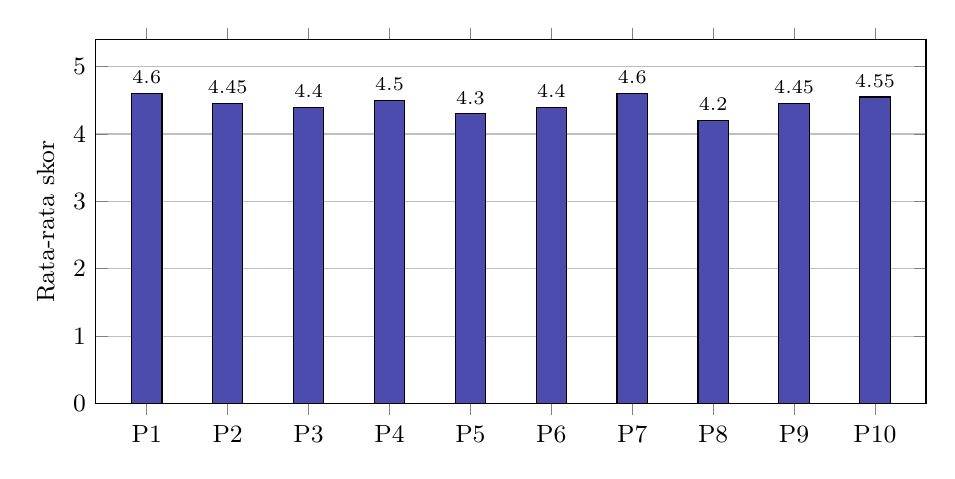
\begin{tikzpicture}
\begin{axis}[ybar,width=\linewidth,height=6.2cm,bar width=11pt,ymin=0,ymax=5.4,ytick={0,1,2,3,4,5},symbolic x coords={P1,P2,P3,P4,P5,P6,P7,P8,P9,P10},xtick=data,ylabel={Rata-rata skor},nodes near coords,nodes near coords style={font=\scriptsize,/pgf/number format/fixed,/pgf/number format/precision=2},enlarge x limits=0.07,ymajorgrids,tick label style={font=\small},label style={font=\small}]
\addplot[fill=blue!55!black!70] coordinates {(P1,4.60) (P2,4.45) (P3,4.40) (P4,4.50) (P5,4.30) (P6,4.40) (P7,4.60) (P8,4.20) (P9,4.45) (P10,4.55)};
\end{axis}
\end{tikzpicture}
\caption{Rata-rata Penilaian Kuesioner Siswa per Pertanyaan (n=20)}\label{fig:4.1}
\end{figure}

\begin{figure}[H]
\centering
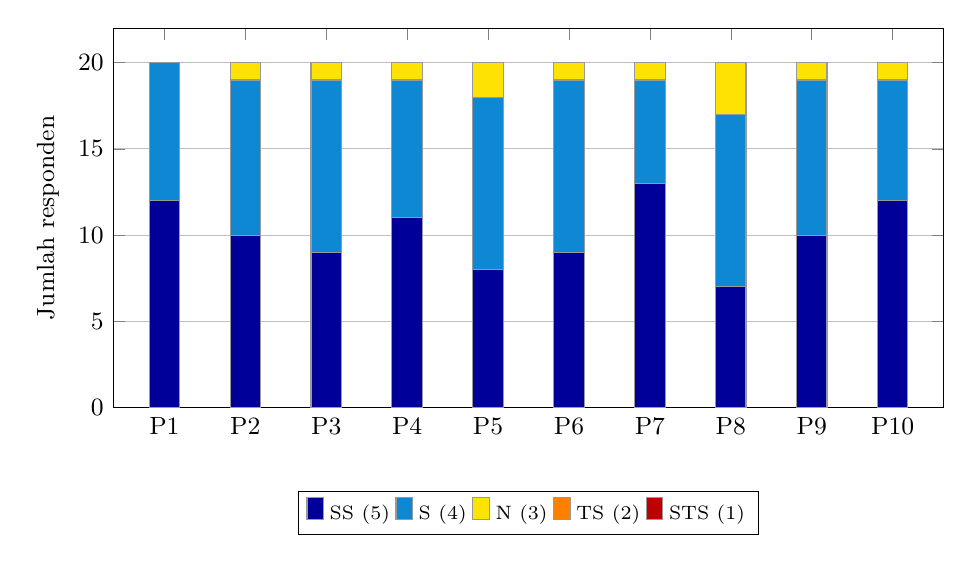
\begin{tikzpicture}
\begin{axis}[ybar stacked,width=\linewidth,height=6.4cm,bar width=11pt,ymin=0,symbolic x coords={P1,P2,P3,P4,P5,P6,P7,P8,P9,P10},xtick=data,ylabel={Jumlah responden},enlarge x limits=0.07,ymajorgrids,legend style={at={(0.5,-0.22)},anchor=north,legend columns=5,font=\scriptsize},tick label style={font=\small},label style={font=\small}]
\addplot[fill=blue!60!black,draw=black!40] coordinates {(P1,12) (P2,10) (P3,9) (P4,11) (P5,8) (P6,9) (P7,13) (P8,7) (P9,10) (P10,12)};
\addplot[fill=cyan!70!blue,draw=black!40] coordinates {(P1,8) (P2,9) (P3,10) (P4,8) (P5,10) (P6,10) (P7,6) (P8,10) (P9,9) (P10,7)};
\addplot[fill=yellow!85!orange,draw=black!40] coordinates {(P1,0) (P2,1) (P3,1) (P4,1) (P5,2) (P6,1) (P7,1) (P8,3) (P9,1) (P10,1)};
\addplot[fill=orange,draw=black!40] coordinates {(P1,0) (P2,0) (P3,0) (P4,0) (P5,0) (P6,0) (P7,0) (P8,0) (P9,0) (P10,0)};
\addplot[fill=red!75!black,draw=black!40] coordinates {(P1,0) (P2,0) (P3,0) (P4,0) (P5,0) (P6,0) (P7,0) (P8,0) (P9,0) (P10,0)};
\legend{SS (5),S (4),N (3),TS (2),STS (1)}
\end{axis}
\end{tikzpicture}
\caption{Distribusi Jawaban Kuesioner Siswa per Pertanyaan (n=20)}\label{fig:4.2}
\end{figure}

Berdasarkan Gambar~\ref{fig:4.1} dan~\ref{fig:4.2}, seluruh pertanyaan mendapatkan nilai rata-rata di atas 4,00 yang berarti seluruh aspek dinilai minimal Baik oleh responden siswa. Aspek yang mendapatkan skor tertinggi adalah kemudahan antarmuka dan manfaat sistem dalam mengurangi keterlambatan laporan (4,60), sedangkan skor terendah diperoleh oleh aspek tampilan desain antarmuka (4,20). Beberapa saran yang diterima dari responden siswa antara lain:

\begin{itemize}
\item Peningkatan desain antarmuka agar lebih modern dan menarik
\item Penambahan fitur notifikasi pengingat untuk pengisian logbook
\item Pengembangan aplikasi mobile untuk memudahkan pengisian logbook dari smartphone
\item Penambahan fitur galeri foto kegiatan dalam logbook
\end{itemize}

\subsection{HASIL KUESIONER GURU (PEMBIMBING DAN KOORDINATOR)}

Kuesioner juga disebarkan kepada 5 orang guru yang berperan sebagai Guru Pembimbing dan Koordinator PKL. Hasil penilaian disajikan pada Tabel~\ref{tab:4.11}.

{\singlespacing\small\renewcommand{\arraystretch}{1.25}
\begin{longtable}{|>{\raggedright\arraybackslash}p{\dimexpr(\linewidth-10\arrayrulewidth)*450/7938-2\tabcolsep\relax}|>{\raggedright\arraybackslash}p{\dimexpr(\linewidth-10\arrayrulewidth)*2092/7938-2\tabcolsep\relax}|>{\raggedright\arraybackslash}p{\dimexpr(\linewidth-10\arrayrulewidth)*605/7938-2\tabcolsep\relax}|>{\raggedright\arraybackslash}p{\dimexpr(\linewidth-10\arrayrulewidth)*590/7938-2\tabcolsep\relax}|>{\raggedright\arraybackslash}p{\dimexpr(\linewidth-10\arrayrulewidth)*590/7938-2\tabcolsep\relax}|>{\raggedright\arraybackslash}p{\dimexpr(\linewidth-10\arrayrulewidth)*605/7938-2\tabcolsep\relax}|>{\raggedright\arraybackslash}p{\dimexpr(\linewidth-10\arrayrulewidth)*619/7938-2\tabcolsep\relax}|>{\raggedright\arraybackslash}p{\dimexpr(\linewidth-10\arrayrulewidth)*1227/7938-2\tabcolsep\relax}|>{\raggedright\arraybackslash}p{\dimexpr(\linewidth-10\arrayrulewidth)*1160/7938-2\tabcolsep\relax}|}
\caption{Hasil Kuesioner Kepuasan Guru (n=5)}\label{tab:4.11}\\
\hline
\rowcolor[HTML]{D9D9D9}\multicolumn{1}{|>{\centering\arraybackslash\bfseries}p{\dimexpr(\linewidth-10\arrayrulewidth)*450/7938-2\tabcolsep\relax}|}{No} & \multicolumn{1}{|>{\centering\arraybackslash\bfseries}p{\dimexpr(\linewidth-10\arrayrulewidth)*2092/7938-2\tabcolsep\relax}|}{Pertanyaan} & \multicolumn{1}{|>{\centering\arraybackslash\bfseries}p{\dimexpr(\linewidth-10\arrayrulewidth)*605/7938-2\tabcolsep\relax}|}{SS (5)} & \multicolumn{1}{|>{\centering\arraybackslash\bfseries}p{\dimexpr(\linewidth-10\arrayrulewidth)*590/7938-2\tabcolsep\relax}|}{S (4)} & \multicolumn{1}{|>{\centering\arraybackslash\bfseries}p{\dimexpr(\linewidth-10\arrayrulewidth)*590/7938-2\tabcolsep\relax}|}{N (3)} & \multicolumn{1}{|>{\centering\arraybackslash\bfseries}p{\dimexpr(\linewidth-10\arrayrulewidth)*605/7938-2\tabcolsep\relax}|}{TS (2)} & \multicolumn{1}{|>{\centering\arraybackslash\bfseries}p{\dimexpr(\linewidth-10\arrayrulewidth)*619/7938-2\tabcolsep\relax}|}{STS (1)} & \multicolumn{1}{|>{\centering\arraybackslash\bfseries}p{\dimexpr(\linewidth-10\arrayrulewidth)*1227/7938-2\tabcolsep\relax}|}{Rata-rata} & \multicolumn{1}{|>{\centering\arraybackslash\bfseries}p{\dimexpr(\linewidth-10\arrayrulewidth)*1160/7938-2\tabcolsep\relax}|}{Kategori} \\ \hline
\endfirsthead
\hline
\rowcolor[HTML]{D9D9D9}\multicolumn{1}{|>{\centering\arraybackslash\bfseries}p{\dimexpr(\linewidth-10\arrayrulewidth)*450/7938-2\tabcolsep\relax}|}{No} & \multicolumn{1}{|>{\centering\arraybackslash\bfseries}p{\dimexpr(\linewidth-10\arrayrulewidth)*2092/7938-2\tabcolsep\relax}|}{Pertanyaan} & \multicolumn{1}{|>{\centering\arraybackslash\bfseries}p{\dimexpr(\linewidth-10\arrayrulewidth)*605/7938-2\tabcolsep\relax}|}{SS (5)} & \multicolumn{1}{|>{\centering\arraybackslash\bfseries}p{\dimexpr(\linewidth-10\arrayrulewidth)*590/7938-2\tabcolsep\relax}|}{S (4)} & \multicolumn{1}{|>{\centering\arraybackslash\bfseries}p{\dimexpr(\linewidth-10\arrayrulewidth)*590/7938-2\tabcolsep\relax}|}{N (3)} & \multicolumn{1}{|>{\centering\arraybackslash\bfseries}p{\dimexpr(\linewidth-10\arrayrulewidth)*605/7938-2\tabcolsep\relax}|}{TS (2)} & \multicolumn{1}{|>{\centering\arraybackslash\bfseries}p{\dimexpr(\linewidth-10\arrayrulewidth)*619/7938-2\tabcolsep\relax}|}{STS (1)} & \multicolumn{1}{|>{\centering\arraybackslash\bfseries}p{\dimexpr(\linewidth-10\arrayrulewidth)*1227/7938-2\tabcolsep\relax}|}{Rata-rata} & \multicolumn{1}{|>{\centering\arraybackslash\bfseries}p{\dimexpr(\linewidth-10\arrayrulewidth)*1160/7938-2\tabcolsep\relax}|}{Kategori} \\ \hline
\endhead
1 & Sistem mudah dipahami dan digunakan oleh guru & 3 & 2 & 0 & 0 & 0 & 4,60 & Sangat Baik \\ \hline
2 & Fitur monitoring logbook (self-reporting) mempermudah proses pengawasan siswa & 4 & 1 & 0 & 0 & 0 & 4,80 & Sangat Baik \\ \hline
3 & Monitoring progres siswa dapat dilakukan secara real-time & 3 & 2 & 0 & 0 & 0 & 4,60 & Sangat Baik \\ \hline
4 & Proses penilaian akhir siswa lebih efisien dibanding cara manual & 4 & 1 & 0 & 0 & 0 & 4,80 & Sangat Baik \\ \hline
5 & Sistem sesuai dengan kebutuhan pengelolaan PKL di SMK PGRI Telagasari & 3 & 2 & 0 & 0 & 0 & 4,60 & Sangat Baik \\ \hline
6 & Fitur rekapitulasi dan ekspor laporan sangat membantu & 3 & 2 & 0 & 0 & 0 & 4,60 & Sangat Baik \\ \hline
7 & Sistem berpotensi meningkatkan efisiensi administrasi PKL secara keseluruhan & 4 & 1 & 0 & 0 & 0 & 4,80 & Sangat Baik \\ \hline
\end{longtable}}

Seluruh responden guru memberikan penilaian dalam kategori Sangat Baik dengan rata-rata keseluruhan mencapai 4,69. Hasil tersebut divisualisasikan melalui grafik berikut.

\begin{figure}[H]
\centering
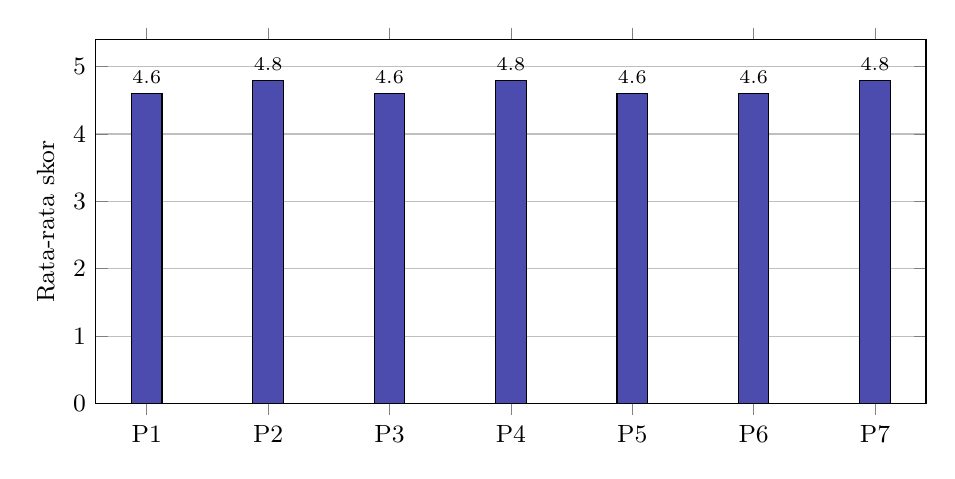
\begin{tikzpicture}
\begin{axis}[ybar,width=\linewidth,height=6.2cm,bar width=11pt,ymin=0,ymax=5.4,ytick={0,1,2,3,4,5},symbolic x coords={P1,P2,P3,P4,P5,P6,P7},xtick=data,ylabel={Rata-rata skor},nodes near coords,nodes near coords style={font=\scriptsize,/pgf/number format/fixed,/pgf/number format/precision=2},enlarge x limits=0.07,ymajorgrids,tick label style={font=\small},label style={font=\small}]
\addplot[fill=blue!55!black!70] coordinates {(P1,4.60) (P2,4.80) (P3,4.60) (P4,4.80) (P5,4.60) (P6,4.60) (P7,4.80)};
\end{axis}
\end{tikzpicture}
\caption{Rata-rata Penilaian Kuesioner Guru per Pertanyaan (n=5)}\label{fig:4.3}
\end{figure}

Berdasarkan Gambar~\ref{fig:4.3}, seluruh pertanyaan mendapatkan nilai rata-rata di atas 4,50. Fitur monitoring logbook, proses penilaian akhir siswa, dan potensi peningkatan efisiensi administrasi mendapatkan skor tertinggi sebesar 4,80. Para guru menyatakan bahwa sistem InternSync sangat membantu dalam menyederhanakan proses monitoring kegiatan PKL siswa. Saran yang diterima antara lain:

\begin{itemize}
\item Penambahan fitur push notification agar pembimbing lebih cepat mengetahui logbook baru dan izin yang perlu ditinjau
\item Pengembangan fitur untuk melampirkan dokumentasi kunjungan industri oleh pembimbing
\item Penyempurnaan fitur ekspor laporan agar dapat dikustomisasi sesuai format administrasi sekolah
\end{itemize}

\subsection{PERBANDINGAN HASIL KUESIONER SISWA DAN GURU}

Untuk mendapatkan gambaran menyeluruh mengenai tingkat kepuasan pengguna, Gambar~\ref{fig:4.4} membandingkan rata-rata keseluruhan skor kuesioner siswa dan guru. Nilai rata-rata diambil dari rekapitulasi kuesioner pada Tabel~\ref{tab:4.10} dan Tabel~\ref{tab:4.11}.

\begin{figure}[H]
\centering
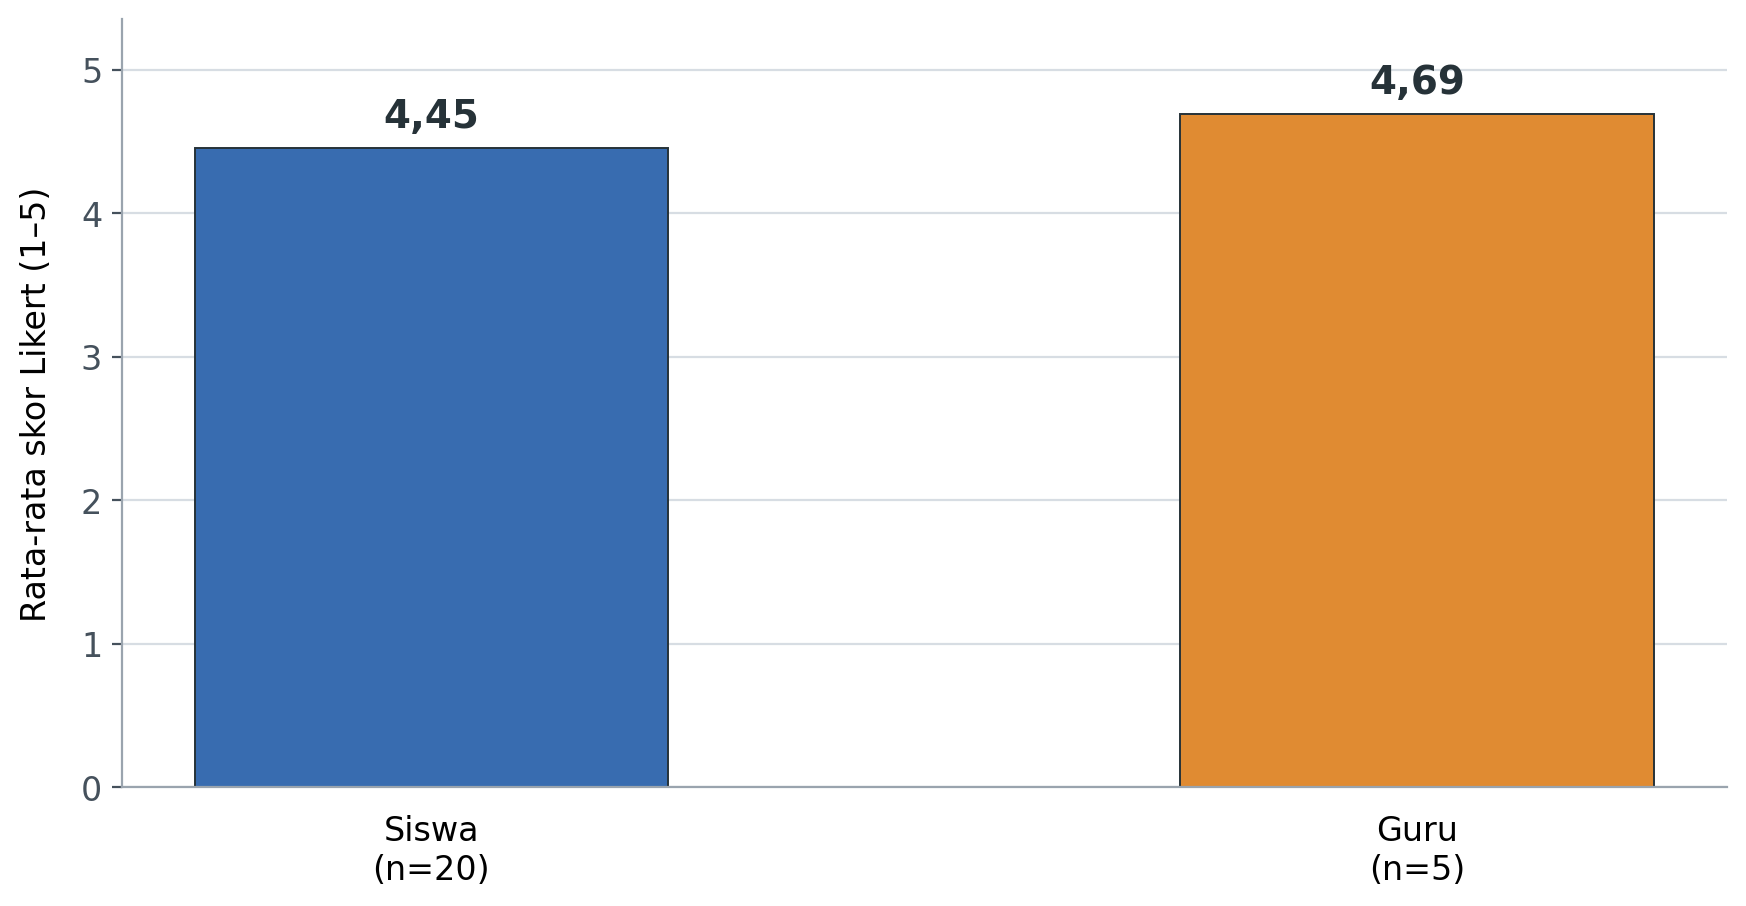
\includegraphics[width=0.85\linewidth]{gambar/grafik-4-4.png}
\caption{Perbandingan Rata-rata Keseluruhan Kuesioner Siswa dan Guru}\label{fig:4.4}
\end{figure}

Berdasarkan Gambar~\ref{fig:4.4}, rata-rata penilaian siswa adalah 4,45, sedangkan rata-rata penilaian guru adalah 4,69. Kedua nilai tersebut termasuk dalam kategori Sangat Baik. Rata-rata guru lebih tinggi 0,24 poin daripada rata-rata siswa. Perbandingan ini menggunakan skor keseluruhan tiap kelompok; jumlah dan butir pertanyaan pada kuesioner siswa dan guru berbeda, sehingga grafik tidak dimaksudkan sebagai perbandingan langsung untuk setiap aspek.

\section{REKAPITULASI HASIL PENGUJIAN}

Berdasarkan seluruh pengujian yang telah dilakukan, berikut adalah rekapitulasi hasil pengujian sistem InternSync secara keseluruhan yang disajikan pada Tabel~\ref{tab:4.12}.

{\singlespacing\small\renewcommand{\arraystretch}{1.25}
\begin{longtable}{|>{\raggedright\arraybackslash}p{\dimexpr(\linewidth-6\arrayrulewidth)*527/7938-2\tabcolsep\relax}|>{\raggedright\arraybackslash}p{\dimexpr(\linewidth-6\arrayrulewidth)*3288/7938-2\tabcolsep\relax}|>{\centering\arraybackslash}p{\dimexpr(\linewidth-6\arrayrulewidth)*975/7938-2\tabcolsep\relax}|>{\centering\arraybackslash}p{\dimexpr(\linewidth-6\arrayrulewidth)*1424/7938-2\tabcolsep\relax}|>{\centering\arraybackslash}p{\dimexpr(\linewidth-6\arrayrulewidth)*1724/7938-2\tabcolsep\relax}|}
\caption{Rekapitulasi Hasil Pengujian Sistem InternSync}\label{tab:4.12}\\
\hline
\rowcolor[HTML]{D9D9D9}\multicolumn{1}{|>{\centering\arraybackslash\bfseries}p{\dimexpr(\linewidth-6\arrayrulewidth)*527/7938-2\tabcolsep\relax}|}{No} & \multicolumn{1}{|>{\centering\arraybackslash\bfseries}p{\dimexpr(\linewidth-6\arrayrulewidth)*3288/7938-2\tabcolsep\relax}|}{Parameter Pengujian} & \multicolumn{1}{|>{\centering\arraybackslash\bfseries}p{\dimexpr(\linewidth-6\arrayrulewidth)*975/7938-2\tabcolsep\relax}|}{Total} & \multicolumn{1}{|>{\centering\arraybackslash\bfseries}p{\dimexpr(\linewidth-6\arrayrulewidth)*1424/7938-2\tabcolsep\relax}|}{Berhasil} & \multicolumn{1}{|>{\centering\arraybackslash\bfseries}p{\dimexpr(\linewidth-6\arrayrulewidth)*1724/7938-2\tabcolsep\relax}|}{Persentase} \\ \hline
\endfirsthead
\hline
\rowcolor[HTML]{D9D9D9}\multicolumn{1}{|>{\centering\arraybackslash\bfseries}p{\dimexpr(\linewidth-6\arrayrulewidth)*527/7938-2\tabcolsep\relax}|}{No} & \multicolumn{1}{|>{\centering\arraybackslash\bfseries}p{\dimexpr(\linewidth-6\arrayrulewidth)*3288/7938-2\tabcolsep\relax}|}{Parameter Pengujian} & \multicolumn{1}{|>{\centering\arraybackslash\bfseries}p{\dimexpr(\linewidth-6\arrayrulewidth)*975/7938-2\tabcolsep\relax}|}{Total} & \multicolumn{1}{|>{\centering\arraybackslash\bfseries}p{\dimexpr(\linewidth-6\arrayrulewidth)*1424/7938-2\tabcolsep\relax}|}{Berhasil} & \multicolumn{1}{|>{\centering\arraybackslash\bfseries}p{\dimexpr(\linewidth-6\arrayrulewidth)*1724/7938-2\tabcolsep\relax}|}{Persentase} \\ \hline
\endhead
1 & Fungsionalitas Peran Siswa & 10 & 10 & 100\% \\ \hline
2 & Fungsionalitas Peran Guru Pembimbing & 9 & 9 & 100\% \\ \hline
3 & Fungsionalitas Peran Koordinator PKL & 12 & 12 & 100\% \\ \hline
4 & Fungsionalitas Peran Hubin & 10 & 10 & 100\% \\ \hline
5 & Fungsionalitas Peran Admin Sistem & 6 & 6 & 100\% \\ \hline
6 & Keamanan Akses (RBAC) & 5 & 5 & 100\% \\ \hline
7 & Penanganan Kesalahan (Error Handling) & 6 & 6 & 100\% \\ \hline
8 & Responsivitas Antarmuka & 5 & 5 & 100\% \\ \hline
 & \textbf{Total Keseluruhan} & \textbf{63} & \textbf{63} & \textbf{100\%} \\ \hline
\end{longtable}}

Berdasarkan hasil rekapitulasi pada Tabel~\ref{tab:4.12}, dari total 63 skenario pengujian pada delapan parameter, seluruh skenario berhasil dijalankan dengan hasil yang sesuai. Parameter ke-9, yaitu kuesioner kepuasan pengguna, dibahas pada subbab 4.8 dan tidak dihitung sebagai skenario Black Box karena berupa penilaian subjektif. Tingkat keberhasilan 100\% pada seluruh parameter pengujian menunjukkan bahwa sistem InternSync siap diimplementasikan di lingkungan SMK PGRI Telagasari melalui domain \url{https://internsync.smkpgritelagasari.sch.id/.}
